% Options for packages loaded elsewhere
\PassOptionsToPackage{unicode}{hyperref}
\PassOptionsToPackage{hyphens}{url}
%
\documentclass[
]{book}
\usepackage{lmodern}
\usepackage{amsmath}
\usepackage{ifxetex,ifluatex}
\ifnum 0\ifxetex 1\fi\ifluatex 1\fi=0 % if pdftex
  \usepackage[T1]{fontenc}
  \usepackage[utf8]{inputenc}
  \usepackage{textcomp} % provide euro and other symbols
  \usepackage{amssymb}
\else % if luatex or xetex
  \usepackage{unicode-math}
  \defaultfontfeatures{Scale=MatchLowercase}
  \defaultfontfeatures[\rmfamily]{Ligatures=TeX,Scale=1}
\fi
% Use upquote if available, for straight quotes in verbatim environments
\IfFileExists{upquote.sty}{\usepackage{upquote}}{}
\IfFileExists{microtype.sty}{% use microtype if available
  \usepackage[]{microtype}
  \UseMicrotypeSet[protrusion]{basicmath} % disable protrusion for tt fonts
}{}
\makeatletter
\@ifundefined{KOMAClassName}{% if non-KOMA class
  \IfFileExists{parskip.sty}{%
    \usepackage{parskip}
  }{% else
    \setlength{\parindent}{0pt}
    \setlength{\parskip}{6pt plus 2pt minus 1pt}}
}{% if KOMA class
  \KOMAoptions{parskip=half}}
\makeatother
\usepackage{xcolor}
\IfFileExists{xurl.sty}{\usepackage{xurl}}{} % add URL line breaks if available
\IfFileExists{bookmark.sty}{\usepackage{bookmark}}{\usepackage{hyperref}}
\hypersetup{
  pdftitle={Anuario Estadístico 2019},
  pdfauthor={Caja de Salud de la Banca Privada},
  hidelinks,
  pdfcreator={LaTeX via pandoc}}
\urlstyle{same} % disable monospaced font for URLs
\usepackage{longtable,booktabs}
\usepackage{calc} % for calculating minipage widths
% Correct order of tables after \paragraph or \subparagraph
\usepackage{etoolbox}
\makeatletter
\patchcmd\longtable{\par}{\if@noskipsec\mbox{}\fi\par}{}{}
\makeatother
% Allow footnotes in longtable head/foot
\IfFileExists{footnotehyper.sty}{\usepackage{footnotehyper}}{\usepackage{footnote}}
\makesavenoteenv{longtable}
\usepackage{graphicx}
\makeatletter
\def\maxwidth{\ifdim\Gin@nat@width>\linewidth\linewidth\else\Gin@nat@width\fi}
\def\maxheight{\ifdim\Gin@nat@height>\textheight\textheight\else\Gin@nat@height\fi}
\makeatother
% Scale images if necessary, so that they will not overflow the page
% margins by default, and it is still possible to overwrite the defaults
% using explicit options in \includegraphics[width, height, ...]{}
\setkeys{Gin}{width=\maxwidth,height=\maxheight,keepaspectratio}
% Set default figure placement to htbp
\makeatletter
\def\fps@figure{htbp}
\makeatother
\setlength{\emergencystretch}{3em} % prevent overfull lines
\providecommand{\tightlist}{%
  \setlength{\itemsep}{0pt}\setlength{\parskip}{0pt}}
\setcounter{secnumdepth}{5}
\usepackage{booktabs}
\ifluatex
  \usepackage{selnolig}  % disable illegal ligatures
\fi
\usepackage[]{natbib}
\bibliographystyle{apalike}

\title{Anuario Estadístico 2019}
\author{Caja de Salud de la Banca Privada}
\date{2021}

\begin{document}
\maketitle

{
\setcounter{tocdepth}{1}
\tableofcontents
}
\hypertarget{poblaciuxf3n}{%
\chapter{Población}\label{poblaciuxf3n}}

asdasd

\begin{table}

\caption{\label{tab:unnamed-chunk-4}Población asegurada, por regional y sexo}
\centering
\begin{tabular}[t]{lrrr}
\toprule
Regional & Femenino & Masculino & Total\\
\midrule
La Paz & 20933 & 18947 & 39880\\
Santa Cruz & 14418 & 16832 & 31250\\
Cochabamba & 9203 & 8204 & 17407\\
Tarija & 2157 & 1819 & 3976\\
Chuquisaca & 1649 & 1784 & 3433\\
\addlinespace
Oruro & 4519 & 1481 & 3050\\
Potosí & 1273 & 1165 & 2438\\
Beni & 1251 & 1162 & 2413\\
Pando & 305 & 264 & 569\\
\bottomrule
\end{tabular}
\end{table}

\begin{figure}
\centering
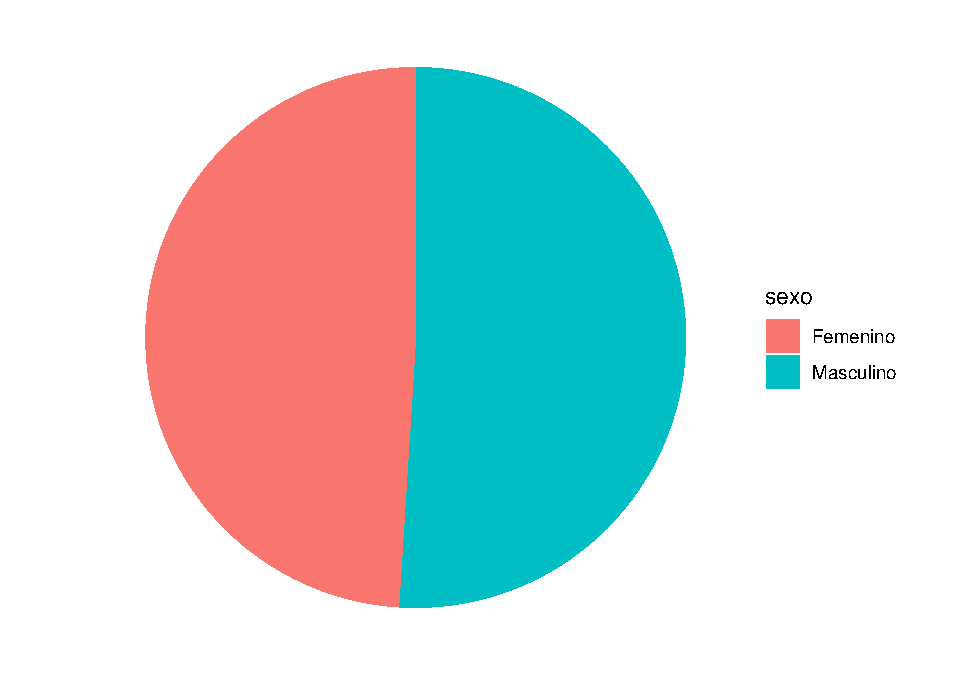
\includegraphics{Anuario2019_files/figure-latex/unnamed-chunk-6-1.pdf}
\caption{\label{fig:unnamed-chunk-6}Distribución porcentual de la Población por sexo}
\end{figure}

\hypertarget{consulta-externa}{%
\chapter{Consulta Externa}\label{consulta-externa}}

\hypertarget{atenciuxf3n-hospitales-egresos}{%
\chapter{Atención Hospitales Egresos}\label{atenciuxf3n-hospitales-egresos}}

\hypertarget{atenciuxf3n-hospitales-cirugias}{%
\chapter{Atención Hospitales Cirugias}\label{atenciuxf3n-hospitales-cirugias}}

\hypertarget{partos-rn}{%
\chapter{Partos RN}\label{partos-rn}}

\hypertarget{medicina-del-trabajo}{%
\chapter{Medicina del trabajo}\label{medicina-del-trabajo}}

  \bibliography{book.bib,packages.bib}

\end{document}
